\documentclass{article}
\usepackage[a4paper, margin=1in]{geometry}
\usepackage{amsmath}
\usepackage{tikz}
\begin{document}
\begin{flushleft}
    

\textbf{\LaTeX}\\ \vspace{11pt}
\textbf{Functions}\\ \vspace{-11pt}
\begin{verbatim}
To define:
\newcommand{\commandName}[numArgs]{
    function definition here
    use #1 to reference the first argument, #2 to reference the second, etc
}

To use:
\commandName{arg1}{arg2}...
This will output the contents of the function's definition
\end{verbatim}

\textbf{Tikz}\\ \vspace{-11pt}
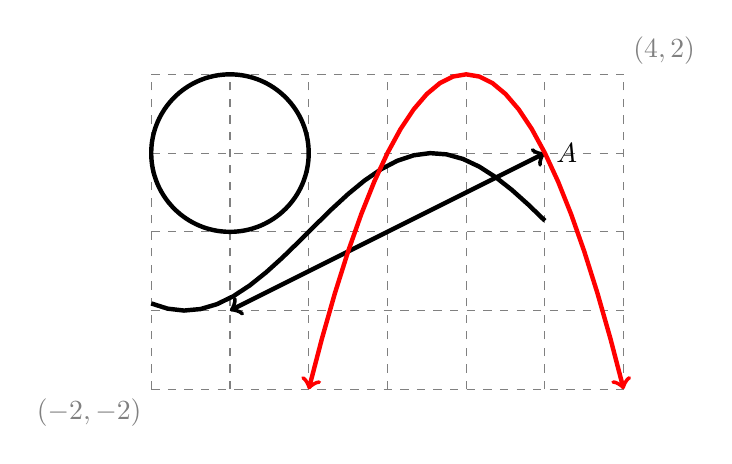
\begin{tikzpicture}
    \draw[dashed, gray] (-2,-2)node[below left]{$(-2,-2)$} grid (4,2)node[above right]{$(4,2)$};
    \draw[ultra thick, <->](-1,-1)--(3,1)node[right]{$A$};
    \draw[ultra thick] (-1,1) circle (1);
    \draw[ultra thick, domain=-2:3] plot (\x, {sin(\x r)});
    \draw[ultra thick, domain=0:4, red, <->] plot (\x, {-(pow(\x,2)-4*\x+2)});
\end{tikzpicture}

This plot was produced by the following:
\begin{verbatim}
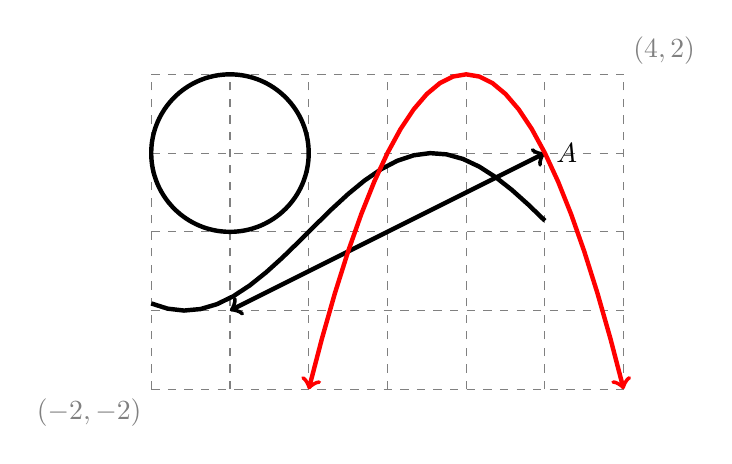
\begin{tikzpicture}
    \draw[dashed, gray] (-2,-2)node[below left]{$(-2,-2)$} grid (4,2)node[above right]{$(4,2)$};
    \draw[ultra thick, <->](-1,-1)--(3,1)node[right]{$A$};
    \draw[ultra thick] (-1,1) circle (1);
    \draw[ultra thick, domain=-2:3] plot (\x, {sin(\x r)});
    \draw[ultra thick, domain=0:4, red, <->] plot (\x, {-(pow(\x,2)-4*\x+2)});
\end{tikzpicture}
\end{verbatim}
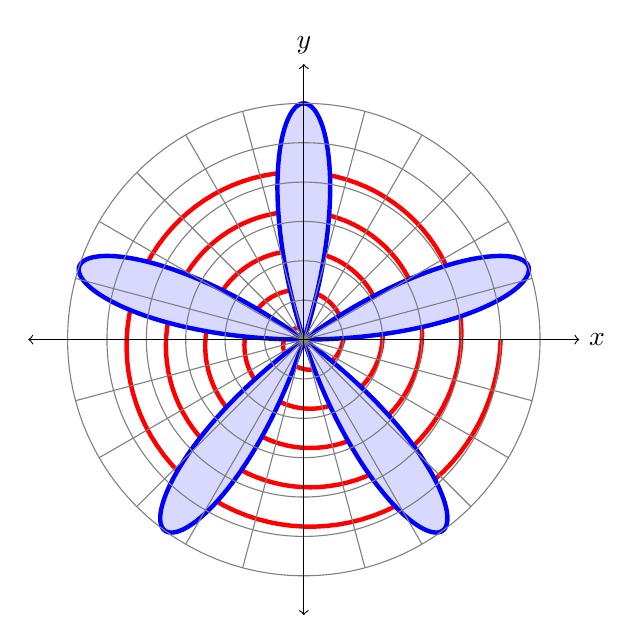
\begin{tikzpicture}[scale=.5]
    \draw[ultra thick, red, domain=0:1800, samples=500] plot(\x: {\x / 360});
    \draw[ultra thick, blue, domain=0:180,samples=500, fill=blue!15] plot (\x: {6*sin(5*\x)});
    \foreach \x in {1, 2, ..., 6}
        \draw[gray] (0,0) circle (\x);
        
    \foreach \a in {15, 30, ..., 345}
        \draw[gray] (0:0) -- (\a:6);
    \draw[<->] (-7,0)--(7,0) node[right]{$x$};
    \draw[<->] (0,-7)--(0,7) node[above]{$y$};

\end{tikzpicture}
\begin{verbatim}
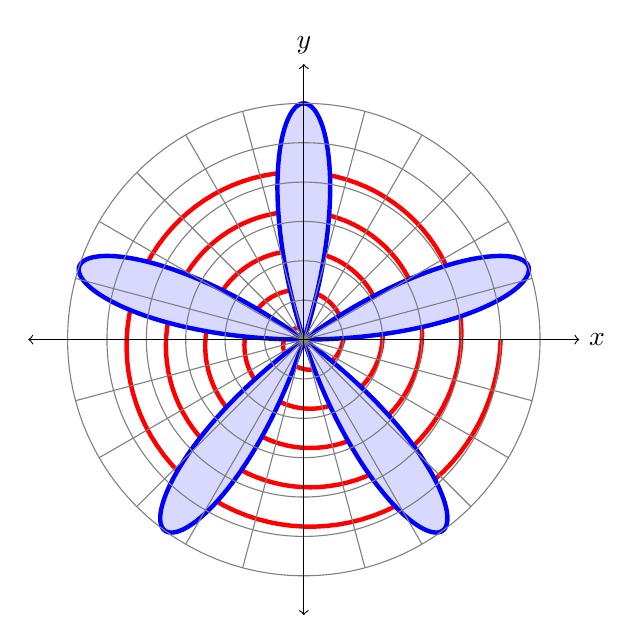
\begin{tikzpicture}[scale=.5]
    \draw[ultra thick, red, domain=0:1800, samples=500] plot(\x: {\x / 360});
    \draw[ultra thick, blue, domain=0:180,samples=500, fill=blue!15] plot (\x: {6*sin(5*\x)});
    \foreach \x in {1, 2, ..., 6}
        \draw[gray] (0,0) circle (\x);
        
    \foreach \a in {15, 30, ..., 345}
        \draw[gray] (0:0) -- (\a:6);
    \draw[<->] (-7,0)--(7,0) node[right]{$x$};
    \draw[<->] (0,-7)--(0,7) node[above]{$y$};
\end{tikzpicture}
\end{verbatim}

\textbf{Links}\\ \vspace{-11pt}
\begin{verbatim}
\href{target}{text} to do a normal hyperlink
\hyperlink{targetName}{text} to link to other locations in the document; the target name should
    be unique; use it in \hypertarget{targetName}{text}
\footnote{footnote text} to insert a footnote; this will generate the correct number where the
    command is and link it to the text in the footer
\end{verbatim}

\textbf{Miscellaneous}\\ \vspace{-11pt}
\begin{verbatim}
\includegraphics[scale=1]{filename.png} to do an image
\begin{tabular}[p|p|p] where p is either l, r, or c (alignment of the column) 
    and | indicates whether or not there's a vertical line
    - use & to separate columns in a line and \\ to separate lines
    - use \hline to draw a horizontal line
\begin{array}[ppp] works similarly
    - must be in math mode (wrap the array in $)
    - I don't think you can have column separators?
\begin{enumerate} makes a numbered list; \begin{itemize} just gives you bullet points
    - use options with enumerate to get custom numbering (roman numerals, alphabet, etc.) 
        - ex. \begin{enumerate}[(a)] to get (a), (b), (c) and so forth
\textit{} is italics, \textbf{} is bold
\hrule makes a horizontal line across the page
\hfill adds as much horizontal whitespace as needed to make the line's contents take up the
whole page
\frac{top}{bottom} makes a fraction, \dfrac{top}{bottom} gives it more vertical space
\newpage and \pagebreak both create new pages (I Think new page spaces the previous page nicely,
    page break breaks it off as is)
\end{verbatim}
\end{flushleft}


\end{document}